\documentclass[crop,tikz]{standalone}
\usetikzlibrary{backgrounds}
\colorlet{blue}{cyan}
\tikzset{
  inverted/.style = {
    color=white,
    background rectangle/.style={fill},
    show background rectangle
  }
}

\tikzset{>=latex}
%\usetikzlibrary{calc,decorations.markings,shapes}
\colorlet{gray}{gray!60}
\colorlet{green}{green}

\begin{document}
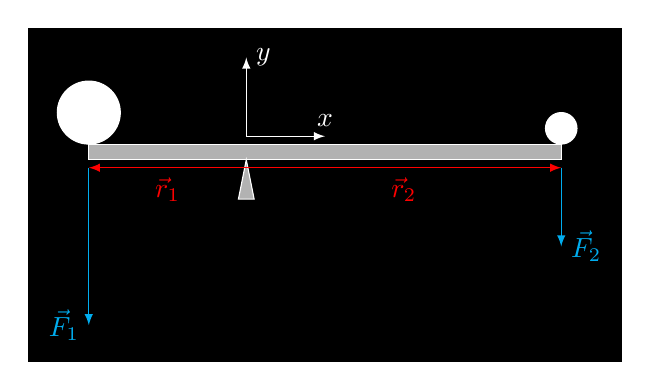
\begin{tikzpicture}[inverted,inverted]
  \draw[fill=gray] (-2,0) rectangle (4,0.2);
  \draw[fill=gray] (-0.1,-0.5) -- (0,0) -- (0.1,-0.5) -- cycle;
  \draw[fill=white] (-2,0.6) circle (0.4);
  \draw[fill=white] ( 4,0.4) circle (0.2);
  \draw[->,red] (0,-0.1) -- node[below]{$\vec{r}_1$} +(-2,0);
  \draw[->,red] (0,-0.1) -- node[below]{$\vec{r}_2$} +( 4,0);
  \draw[->,blue] (-2,-0.1) -- +(0,-2) node[left]{$\vec{F}_{1}$};
  \draw[->,blue] ( 4,-0.1) -- +(0,-1) node[right]{$\vec{F}_{2}$};
  \draw[->] (0,0.3) -- +(1,0) node[above] {$x$};
  \draw[->] (0,0.3) -- +(0,1) node[right] {$y$};
\end{tikzpicture}
\end{document}
